\subsection{Meilenstein 2: Controller Input und GameObject}

Meilenstein 2 stellte die erste Erweiterung der Architektur dar, die das Rendering in Abhängigkeit von User Input ermöglichte. Hierfür wurde \texttt{GameWorld} und \texttt{GameObject} als Klassen eingeführt, deren Semantik sich auch ncoh ind er Abgabeversion findet, aber im Laufe der Arbeit zahlreiche Umbauten erfuhren, von Datencontainern hin zu Fassaden für den Zugriff auf ein ECS.\\

\begin{figure}
    \centering
    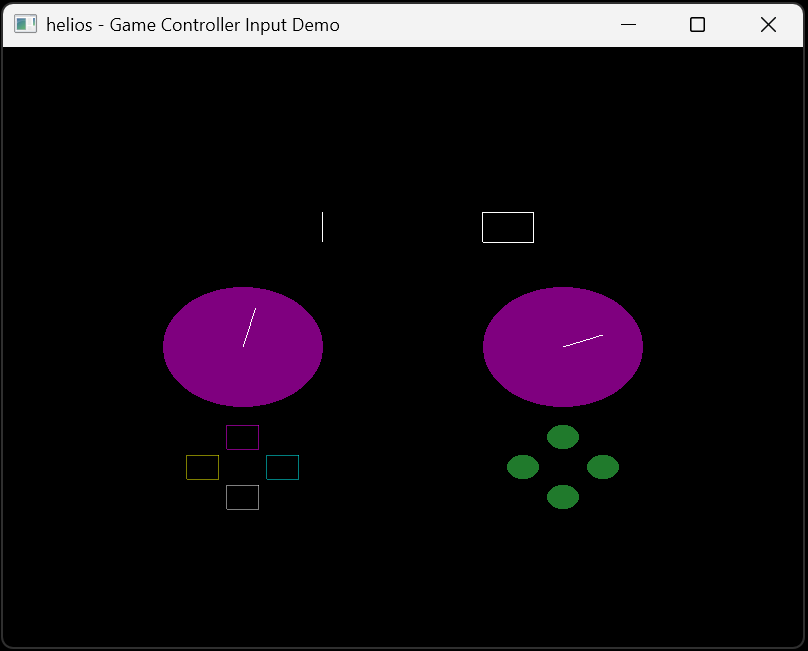
\includegraphics[width=1\columnwidth]{content/de/iterative evolution/img/gamecontrollerinput}
    \caption{Oberfläche der \textit{Game Controller Input Demo}. Der Szenegraph enthält verschiedene geometrische Figuren, deren Fabintensität bzw. Skalierung je nach betätigter Inputs variiert. (Quelle: eigene Aufnahme)}
    \label{fig:gamecontrollerinput}
\end{figure}

\noindent
Die in~\ref{fig:gamecontrollerinput} dargesteltle Demo zeigt die Funktionalität der Controller Input Verarbeitung, die über die \texttt{InputManager} Klasse realisiert wird.
Hierbei werden sowohl Tastatureingaben als auch Gamepad-Inputs verarbeitet, um die Eigenschaften der dargestellten geometrischen Figuren zu verändern - dies geschieht zu diesem Zeitpunkt ohne weitere Abstraktion direkt über die Anpassungen der Szeneknoten mittels \texttt{setScale()} und \texttt{setTranslation()}.\\
Farbänderungen der Figuren erfolgen über Aufrufe auf die Renderables, die an die Szeneknoten gebunden sind.
Hier hatte sich gezeigt, dass der für den Prototypen ausgearbeitete ENtwurf einerseits zu komplex, andererseits zu unflexibel gewesen ist.
Ein Umbau in weniger Objekte (siehe~\ref{fig:renderable}) erlaubt eine klarere Objekthierarchie von geteilten udn wiedervwerwendbaren Material, Mesh und Shader-Instanzen udnd vereint die Komposition in einem \texttt{RenderPrototype}, der von vielen \texttt{Renderables} geteilt werden kann. Zusätzliche optionale Overrides in form von PDOs erlauben eine individuelle Konfiguration der Renderables.\\
Dies Entwurf hat sich als flexibel erwiesen und konnte auch für eine Spezialisierung von Renderables als UI-Text mit geringfügigen Anpassungen beibehalten werden.\\

\noindent
Eingeführt wurde mit diesem Meilenstein außerdem das Modul \texttt{helios.engine.game} zusammen mit der Klasse \texttt{GameWorld}, die als Container für alle GameObjects fungiert, die wiederum die zentralen Akteure innerhalb der \texttt{GameWorld} darstellen.\\
Die Umsetzung ist zu diesem Zeitpunkt noch stark von einem OOP-Ansatz geprägt und beinhaltete folgende Methode:

\vspace{4mm}
\begin{lstlisting}[style=c++style,
    caption={.},
    label=lst:cmake]

    /**
     * @brief Updates all GameObjects in the world for
     *        the current frame.
     */
   void update(float deltaTime) const noexcept;

    /**
     * @brief Adds a GameObject to the world.
     */
   addGameObject(std::unique_ptr<GameObject> gameObject);

    /**
     * @brief Finds a GameObject by its unique identifier.
     */
   GameObject* find(const helios::util::Guid& guid)

\end{lstlisting}


\noindent
Obwohl die API auch im aktuellen Zustand noch die Möglichkeit bietet, GameObjects zu erstellen, zu aktualisieren und zu suchen, sind die darunterliegenden Implementierungen einem hash-basierten Ansatz über die GUID de ECS-System gewichen.
Dies bedeutet auch, dass die \texttt{update()}-Methode nicht länge bestandteil der Gameworld ist: Sie findet sich in der \texttt{GameLoop}, die in individuelle Phasen und ind er Durchführung abhängig vom Zustand der in der Engine konfigurierbaren State Machines sind.\\

\noindent
Die o.a. Game Controller Input Demo wurde dann erweitert zur einer Steuerung eines Triangles.
Zur leichteren Debugging und zum Testen der Parameter der GameObject wurde außerdem ImGui in die Engine integriert, um verschiedene Eigenschaften zur Laufzeit anpassen zu können - darunter auch die Steuerung für die Kameras, deren Konzept hinsichtlich Game Engine Idiomatio erweitert wurde: Mit SzeneNodes, die Kameras kapseln, können nun Kameras an zur VErfolgung von Spielobjekten direkt als Kindknoten im Szenegraph an die entsprechenden Knoten gebunden werden: Zusätzliche wurde eine Unterstützung implementiert, die ie Angabe der Eigenschaften erlaubt, die von der Affinen Transformationsmatrx des elternobjektes geerbet wrden soll. Als Bitmaske erlaubt dies die KOnfiguaration von Skalierung, Rotation udn Translation, wobei für die Kameraknoten die TRanslation die bevorzugte Option ist..


\begin{figure}
    \centering
    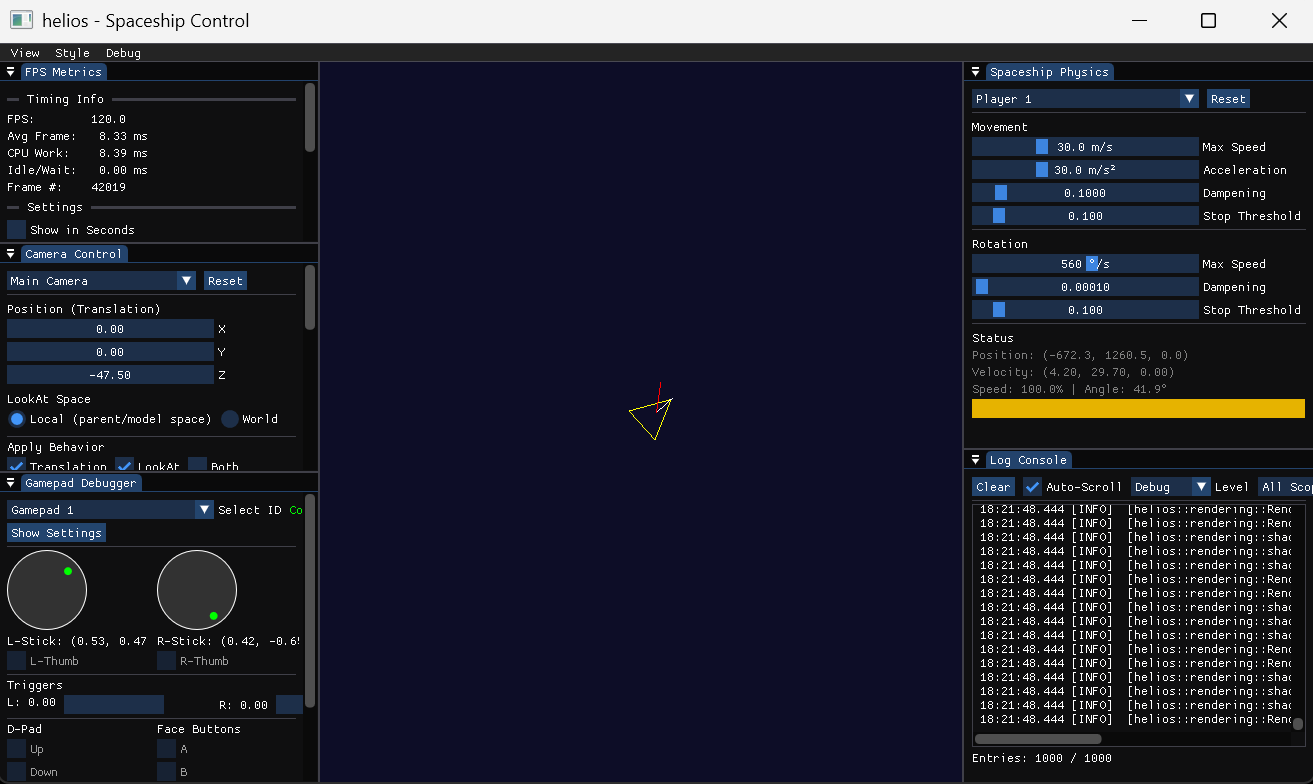
\includegraphics[width=1\columnwidth]{content/de/iterative evolution/img/spaceshipcontrol}
    \caption{Die Spaceship Control Demo beinhaltete neben der Steuerung des Schiffs Imgui Overlays zur Konfiguration verschiedener Welt- und Spielobjektparameter, wie Beschleunigugn und Geschwindigkeit des Spielerschiffes, Kamerapostion sowie eine Anzeige der aktuellen Controlelr Inputs,mit der Möglichkeit die Toleranz (Dead Zone) bzgl. Stick Drift einzustellen. (Quelle: eigene Aufnahme)}
    \label{fig:spaceshipcontrol}
\end{figure}
